\chapter{同时考虑实现型与维持型目标的意图进展}
本章将提出一种基于\SA 的意图调度算法\SAM ,\SAM 支持同时对实现型和维持型目标的调度。其中维持型目标考虑到了在第\ref{background}中提到的被动维持型目标和主动维持型目标。另外,本章对\SAM 的性能在动态和静态环境下进行了实验分析,并与Duff等人提出的PMG\cite{DBLP:conf/atal/DuffHT06}算法进行了比较,实验结果表明\SAM 的表现相对PMG有显著提升。
\subsection{维持型目标}
目前大多数对BDI智能体意图调度方面的研究主要考虑的是实现型目标,即指定某一个智能体要去达到的环境状态,一旦智能体通过执行动作达到了该指定状态,实现型目标即被抛弃。
% MG
但是在许多问题场景中,智能体还必须持续地保持某个环境状态一段时间,例如一个火星探测器必须确保它总是有足够的电池电量用以返回基地充电,否则它可能会因耗尽电池而搁浅。为了避免这种情况,一个理性的智能体需要有一个针对电池的目标,在其电量变得很低之前返回基地充电。这种目标被称为维持型目标,其指定了一个智能体需要持续维持的环境状态。

% Execution

当智能体接收到一个实现型目标时,他将执行一个计划来实现该实现型目标,并在条件实现放弃该目标。
%
然而,对于维持型目标,在其指定的维持条件为假之前,接收该目标不会导致任何动作的执行。而一旦维持条件不满足,智能体就会执行一个计划以修复该维持条件,该行为对应于被动维持型目标;或者当智能体认为该维持条件在不久的将来会不满足时,便会执行一个计划以防止维持条件在环境中失效,该行为则对应于主动维持型目标。只有当智能体不再需要维持条件时,维持型目标才会被抛弃。
% PMG
目前已有一些针对维持型目标的研究方法被提出,Duff\cite{DBLP:conf/atal/DuffHT06}提出了一种基于SI的意图调度方法PMG,该方法可用于决定是否接收一个新的实现型或维持型目标,以及在维持条件满足的情况下,何时采取预防性的措施以防止该维持条件失效。
% more specific
具体地,每次接收到一个新的目标时,智能体都会判断其是否与当前的维持型目标有冲突。如果这个新目标会与一个或多个现有的维持型目标发生冲突,智能体首先会采取预防措施以确保维持型目标在将来不会被破坏,在这之后才去执行该新目标。
% their problem
然而,PMG算法并没有考虑到智能体多个意图间的相互影响。

% AG and MG representation
本章考虑对实现型与维持型目标的调度,以下为其规范表示:
\paragraph{实现型目标}
实现型目标表示智能体想要达到的环境状态,一个实现型目标以一个三元组表示:
$$<G_a,C_g,Pls>$$
其中$G_a$为该目标的名称,$C_g$为目标条件,即一组智能体想要达到的条件。每个目标都与一组用于实现该目标的计划$Pls=\{P_1,\dots,P_n\}$相关联。一旦目标条件被达成,智能体便会抛弃该实现型目标。
\paragraph{维持型目标}
维持型目标定义了某个智能体需要维持的环境状态\cite{DBLP:journals/ci/DuffTH14},一个维持型目标以一个四元组表示:
$$<G_m,C_m,Pls,t>$$
其中$G_m$为该维持型目标的名称,$C_m$为维持条件,$Pls$为一组用于修复该维持条件的计划,$t$为该维持型目标的持续时间(时间结束后该目标就被抛弃)。

和简单的实现型目标不同,根据维持条件$C_m$的破坏能否被可靠地预测,维持型目标可以以不同的方式实现。
\subsubsection{主动维持型目标}
如果维持条件$C_m$何时会被破坏能够被可靠地预测,智能体可以主动地在其被破坏之前执行某个$Pls$中的计划以防止破坏的发生。该设定可能会影响到维持条件$C_m$。例如,如果智能体可以准确地预测智能体执行某个意图的电量消耗,则可以将$C_m$设定为维持电量在零以上。
\subsubsection{被动维持型目标}
另一方面,如果维持条件$C_m$何时会被破坏无法被可靠地预测,智能体可以被动地执行$Pls$中的某个计划,即在$C_m$被破坏之后执行。在这种情况下,维持条件$C_m$的设定需要更保守一些。例如,如果智能体无法准确地预测智能体执行某个意图的电量消耗,则可以将$C_m$设定为一个非零的最小阈值,如20\%。该设定可以确保智能体在维持条件被破坏后有足够的电量返回基地充电。

实际上,主动维持型目标和被动维持型目标是维持型目标应用的两种极端。通常来说,预测机制的可靠程度、效率和破坏维持条件的后果共同决定了该使用哪一种应用方式。

% @TODO problem definition

\subsection{$SA_M$调度算法}
本章介绍同时考虑实现型与维持型目标的意图调度算法\SAM 。\SAM 在第\SA (已在第\ref{SA}章中介绍)的基础上进行拓展,加入对被动与主动维持型目标的考虑。
具体地,\SAM 算法修改了\SA 算法中的扩展与模拟阶段,加入了决定何时以及如何执行修复维持条件的计划的机制,以下是对SA算法的具体修改细节:
\paragraph{对扩展阶段的修改}
% Reactive
在SAM中,被动维持目标和主动维持目标有不同的应对机制。对于被动维持型目标,SAM首先检查被选中的某个拓展节点$N_s$中是否有维持条件被破坏。对于每一个维持条件被破坏的目标,生成一组新的节点,并作为$n_s$的孩子节点。这组节点对应于对应修复计划的执行。也就是说,在$n_s$状态下,智能体可以选择像以往一样继续实现其他目标,也可以选择执行修复计划以重新恢复维持条件。对于被动维持型目标当维持条件没有被破坏时,相关修复计划的执行是被禁止的。
% Proactive
对于主动维持型目标,SAM假定所有维持型目标都处于激活状态,也就是说智能体可以在任何时候都执行维持型目标的相关修复计划,只要当前该相关计划没有在执行状态即可(防止同一个计划的重复执行)。
% Special case for proactive
而当智能体没有任何实现型目标时,若没有维持条件被破坏,则不会有新的节点生成。也就是说,当智能体没有任何目标需要实现时,智能体就会处于等待状态以维持当前的状态。

\paragraph{对模拟阶段的修改}
在模拟阶段,SAM和SA一样,随机选择实现目标过程中可执行的动作执行。当某个被动维持型目标$G_m$被触发时,智能体除了可以选择执行实现型目标,还可以选择执行$G_m$相关的修复计划。而对于主动维持型目标,SAM可以在没有维持型目标相关意图执行时执行其修复计划(避免同一个意图的重复执行)。修复计划同样可以与其他意图交错执行,以避免意图间的冲突以及利用意图间的协同效应。当以下三个条件中的任意一个满足时,模拟阶段即停止:
\begin{enumerate}
  \item 所有的实现型目标都已完成并且没有维持目标被触发。
  \item 当前状态下无法实现剩余的实现型目标。
  \item 所有维持型目标的维持条件在当前状态下都无法修复。
\end{enumerate}

\subsection{实验}
\subsubsection{实验场景介绍}
本章基于一个火星探测器的模拟场景(Mars Rover Simulator)对SAM算法的性能进行评估。该模拟环境为一个网格,由20 $\times$ 20个小方格组成(见图\ref{fig:marsrover})。
\begin{figure}[h!]
\centering
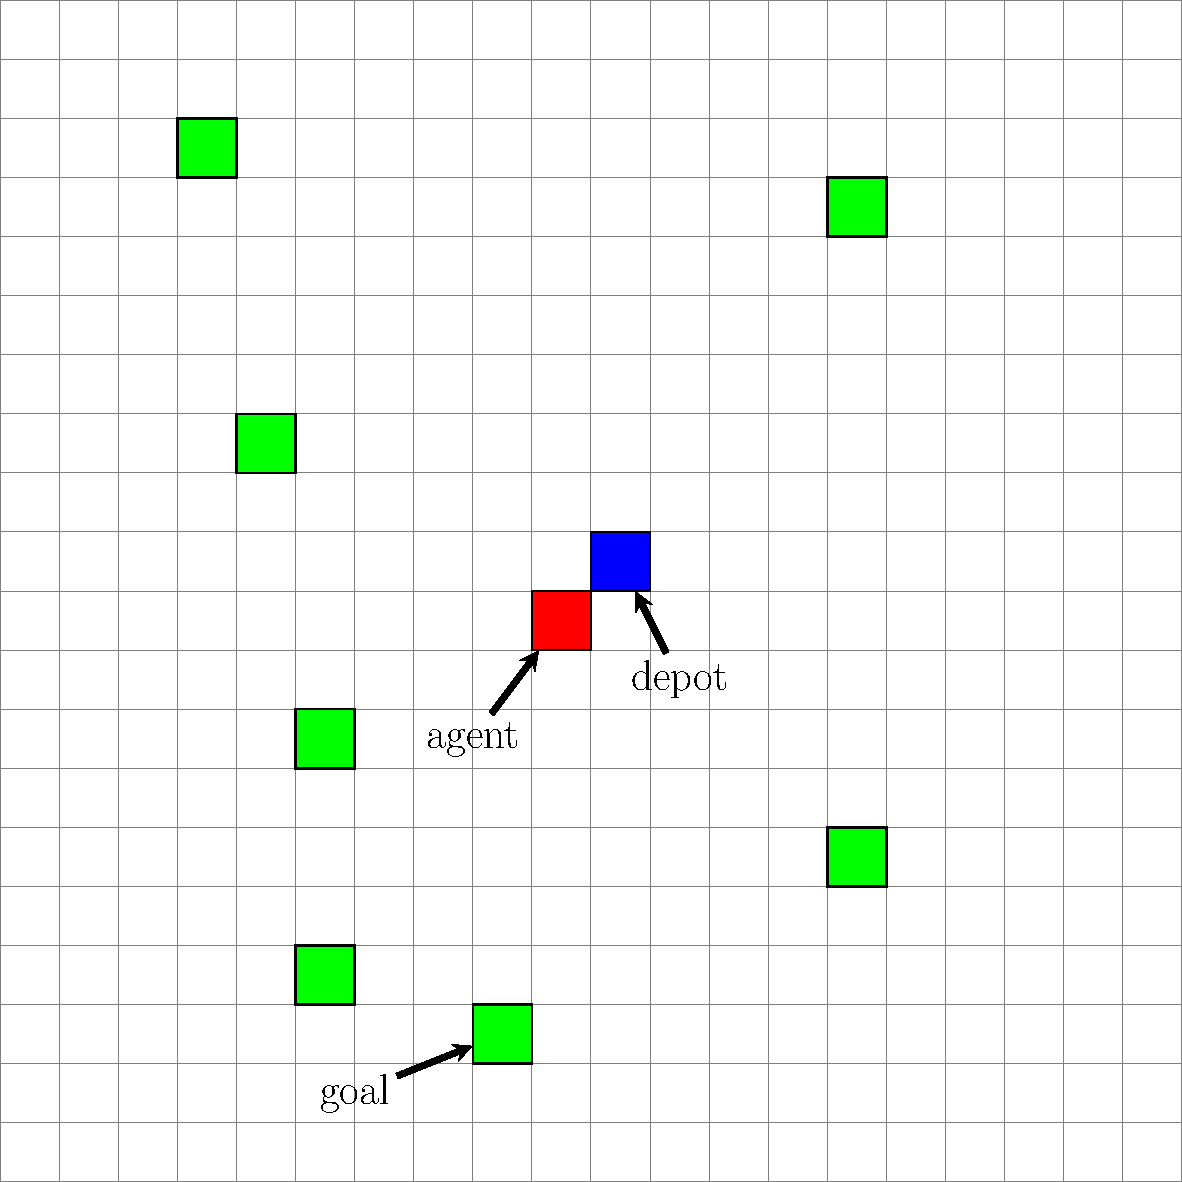
\includegraphics[scale=0.4]{./figs/mg_example}
\captionsetup{justification=centering}
\caption{A Mars rover example}
\label{fig:marsrover}
\end{figure}

% introduction to the Mars rover example
网格中每个方格都是一个智能体可以到达的位置,由(x, y)所表示,其中x和y分别为x坐标与y坐标的值。
%
本实验中假设最左下角的方格坐标为(0, 0),最右上角的方格坐标为(19, 19)。
% 
火星探测器智能体被放置于某个方格中,并按要求以访问网格中某些位置为目标执行相关计划。该智能体一共可以执行4个动作以进行位置的移动:向上移动一个单位,向下移动一个单位,向左移动一个单位以及向右移动一个单位。
% 
另外,每一次的移动都会消耗1点的电量,当电量较低时,智能体可返回基地(10, 10)进行充电(假设基地有无限的电量供应)。
%
该场景下相应的目标计划树可见图\ref{fig:gpt}。
\subsubsection{实验设定}
本文假设在以下所有实验中,智能体每次都从基地出发,其访问的目标地点都是随机生成的\footnote{注意,同一个地点不会生成多个目标}。
% measuring the agent
本实验根据两个标准对智能体性能进行评估:实现目标的数量以及消耗的电池电量。具体地,首先将基于实现目标的数量对智能体进行评估,实现数量越多,性能越好;如果不同的智能体实现目标的数量相同,则将基于电量消耗进行性能评估,消耗电量越低,性能越好。

本文将SAM与Duff等人提出的方法\cite{DBLP:conf/atal/DuffHT06}进行比较,实验考虑到了包含SAM等一共6种方法:

\begin{itemize}
\item \textbf{No maintenance goal (NMG)}: 该方法假设智能体的移动不会消耗电量,因此智能体无需返回基地充电。该方法以FIFO的规则实现目标,在duff 等人的文章ref中有所描述。
\item \textbf{Reactive maintenance goal (RMG)}: 该方法假设智能体无法可靠地预测维持条件何时会被破坏。因此维持型目标的实现方式是被动的,以此确保智能体有足够的电量返回基地充电。当维持型目标被触发时,智能体首先将返回基地充电,然后再尝试实现其他目标。该方法与ref中提到的RMG方法相同。
\item \textbf{Proactive maintenance goal (PMG)}: 该方法假设智能体可以基于SI方法对维持条件的破坏进行可靠的预测。因此,维持型目标的实现方式为主动型。本实验使用 在ref提到的相同方法对维持型目标进行调度。
%
也就是说,在执行其他目标之前,智能体将预测实现该目标的电量消耗情况,如果智能体在实现新目标之后没有足够的电量返回基地,那么将收件执行修复计划以保持充足的电量。
\item \textbf{No maintenance goal MCTS (NMCTS)}: 和NMG类似,该方法假设智能体的移动不会消耗电量。不同的是,实现目标使用的是SA进行调度。
\item \textbf{Reactive maintenance goal MCTS (RMCTS)}: 在该方法设定下,智能体使用SAM进行意图调度,维持型目标的应用方式为被动型。
\item \textbf{Proactive maintenance goal MCTS (PMCTS)}: 和RMCTS类似,该方法使用SAM进行意图调度,不同的是维持型目标的应用方式为被动型。
\end{itemize}

%
为了确保智能体总是有足够的电量用以返回基地,被动维持型目标的维持条件设定为$batteryLevel > 20$。也就是说,即使在(0,0)位置,智能体也总是有足够的电量返回基地(10,10)。
%
对于主动维持型目标,其维持条件设定为$batteryLevel > Distance(agent, depot)$,其中$Distance(agent, depot)$为智能体从当前位置移动到基地所需要消耗的最小电量。
%
一旦维持型目标被触发,其相应的修复计划就会被执行,用以返回基地充电保持或修复维持条件。
%
在以下实验中,SAM和SA的设定为执行100次迭代($\alpha = 100$),每次迭代执行10次的模拟($\beta = 10$)。另外,价值函数设定为$\#goals + \frac{1}{1 + {battery}}$,其中 $\#goals$ 为实现目标的数量, $battery$ 为用以实现目标的消耗电量。

以下实验考虑了动态与静态环境。在以下的实验结果中,本文展示的是每种方法运行100次运行次的平均性能。另外,实际上所有方法都可以在实验中实现所有顶层目标。因此,为了便于分析,本文只使用电池消耗量来衡量不同方法的性能。
\subsubsection{静态环境实验}
在接下来的3个实验中,本文考虑火星探测器智能体在静态环境下的表现。在静态环境下,智能体的所有实现型目标都在初始运行时给定。
\paragraph{Experiment 1}
在第一个实验中,智能体的电池容量被设定为40,智能体需要实现目标的数量从1逐步增加至15。具体实验结果如图\ref{fig:static1}所示。
\begin{figure}[!h]
\centering
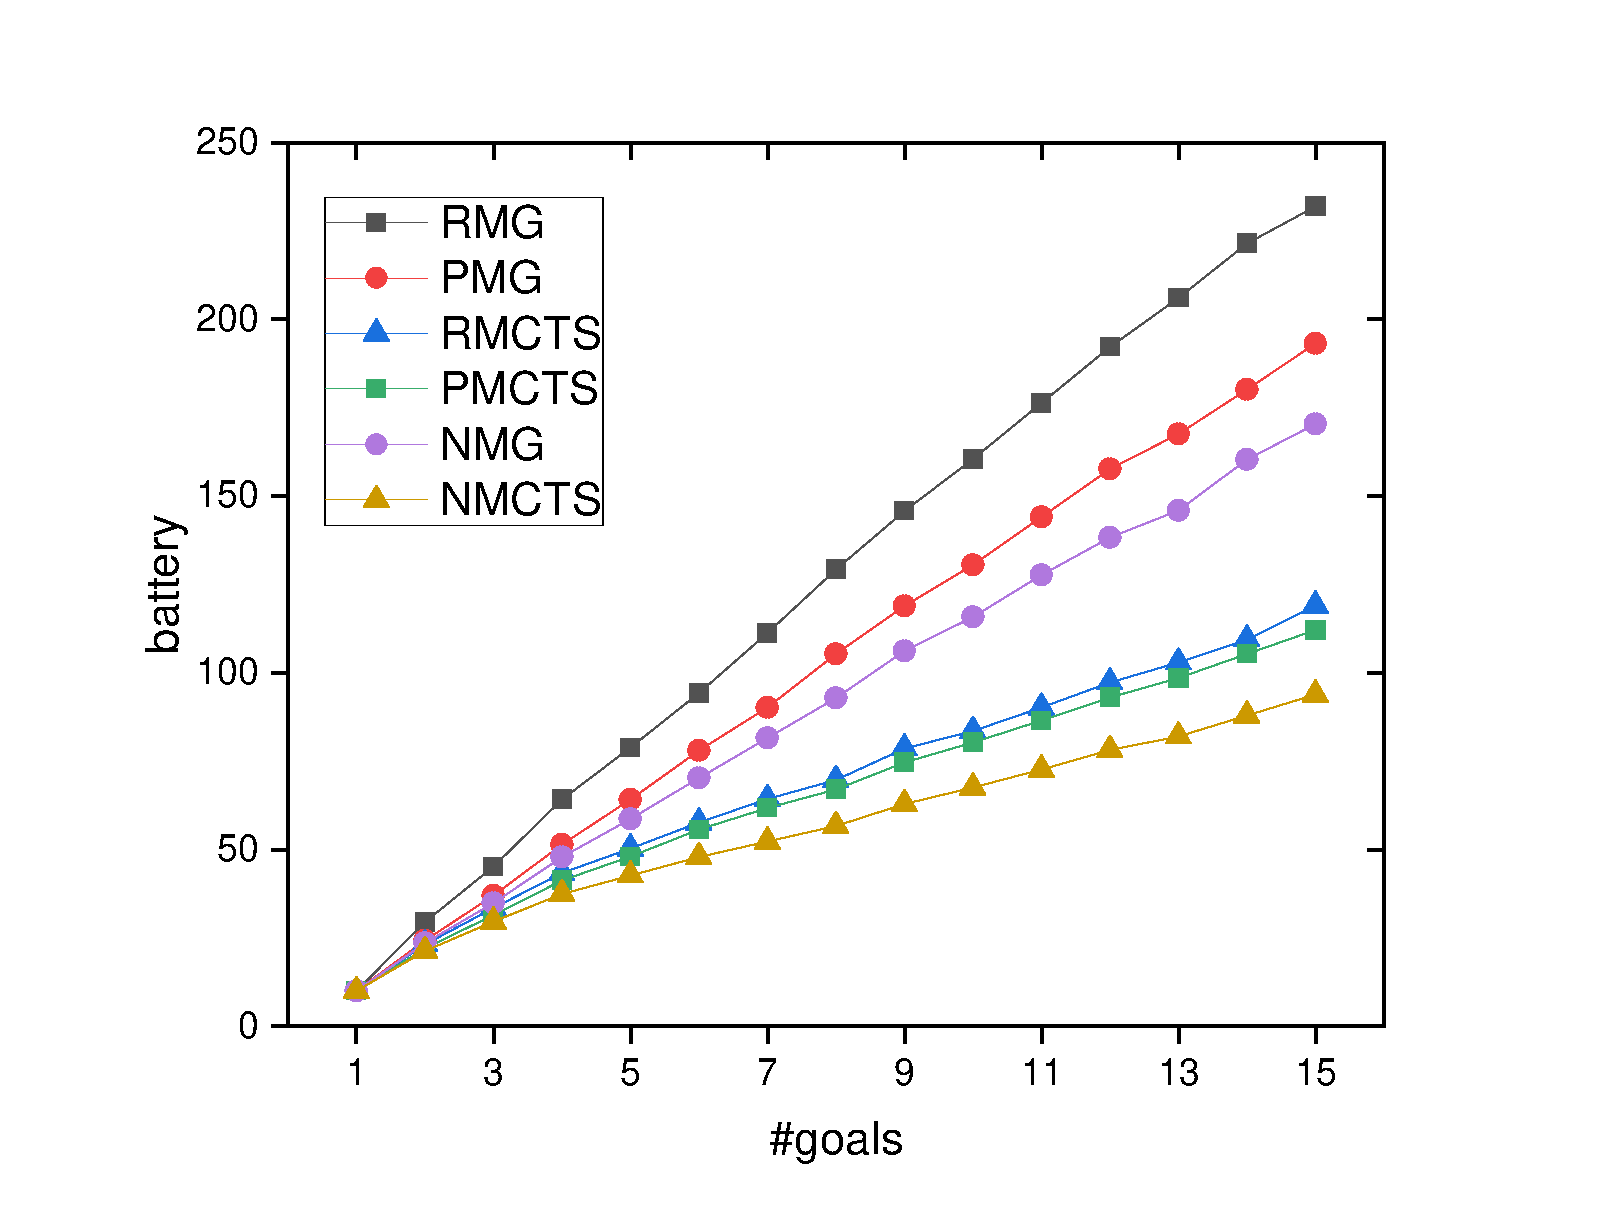
\includegraphics[scale=0.4]{./figs/gX_cY_fixCap40.pdf}
\captionsetup{justification=centering}
\caption{Battery consumptions with fixed capacity of 40}
\label{fig:static1}
\end{figure}

从图中得知,当实现目标数量增加时,所有方法的电量消耗都有所增加。
% two baseline
由于NMCTS和NMG没有电量消耗的考虑,他们可以作为两个基准用以评估其他实际应用方法的性能。
% general
通过分析得知,基于MCTS的方法(NMCTS,PMCTS和RMCTS)性能优于其他方法。另外,使用主动维持型目标的方法的性能表现要优于使用被动维持型目标的方法。
% NMG
在所有测试情况下,RMG的性能表现最差(消耗最多的电量)。
% reason
这是因为NMG仅考虑被动地处理维持型目标,这会导致在点来电量不充足时去实现较远处的目标,导致大量无效的往返移动,浪费电量。
% PMG
相比较之下,PMG表现更好,因为其可以在实现一个目标之前对电量消耗进行评估。如果智能体经过分析后得知其会在实现目标途中触发维持型目标,那么它将首先返回基地充电,再去实现该目标。
% mcts
最后,与PMG和NMG对比,PMG和RMG有着显著的性能优势。特别是当实现目标数量变多时,他们之间的差距也越来越明显。这其中的原因在于基于MCTS的方法不仅仅能够预测维持型目标何时被触发,还能够高效地利用不同意图间的协同效应(智能体可以合并不同意图下的同一个动作以节省电量)。


\paragraph{Experiment 2}
在第二个实验中,智能体的电量被设定为60,其他设定与实验一相同。具体实验结果如图\ref{fig:static2}所示。
\begin{figure}[h!]
\centering
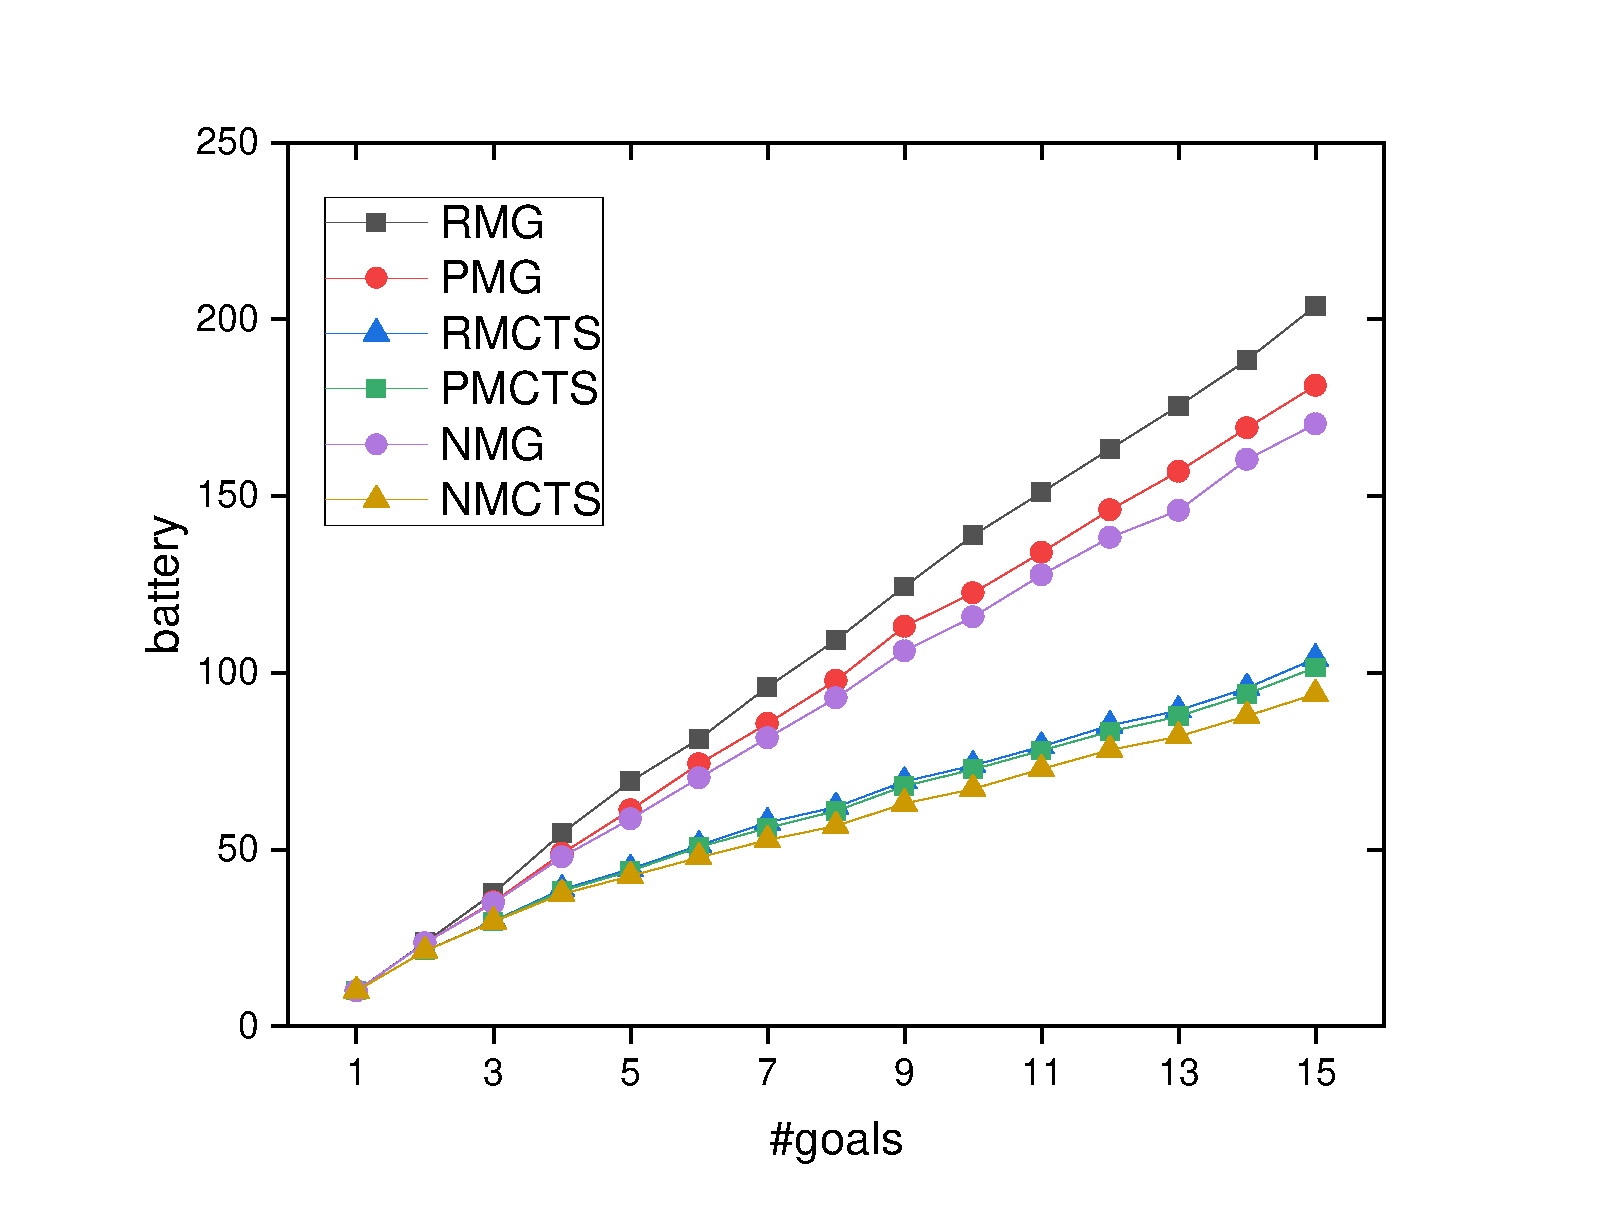
\includegraphics[scale=0.4]{./figs/gX_cY_fixCap60.pdf}
\captionsetup{justification=centering}
\caption{Battery consumptions with fixed tank capacity of 60}
\label{fig:static2}
\end{figure}

从图中得知,当电池容量提升时,所有方法的电量消耗都有所降低。
%
和实验一相似,基于MCTS的方法的性能优于其他方法。在该实验设定下,基于MCTS的方法与非MCTS方法的差距更加显著。这同样也是因为基于MCTS的方法可以更高效地利用不同意图间的协同效应。
%
在实验二中,主动维持型目标的性能同样优于被动维持型目标,但是他们之间的性能差异有所减小。例如,当实现目标的数量为15时,PMCTS的电量消耗仅仅比RMCTS低2.65。
%
这是因为当电池容量变大时,维持型目标被触发的次数减小,使得被动与主动维持型目标直接的差异更小。

\paragraph{Experiment 3}
在第三个实验中,智能体被给定固定10个目标,而电池容量从40改变至200。具体实验结果如图\ref{fig:static4}所示。
\begin{figure}[h!]
\centering
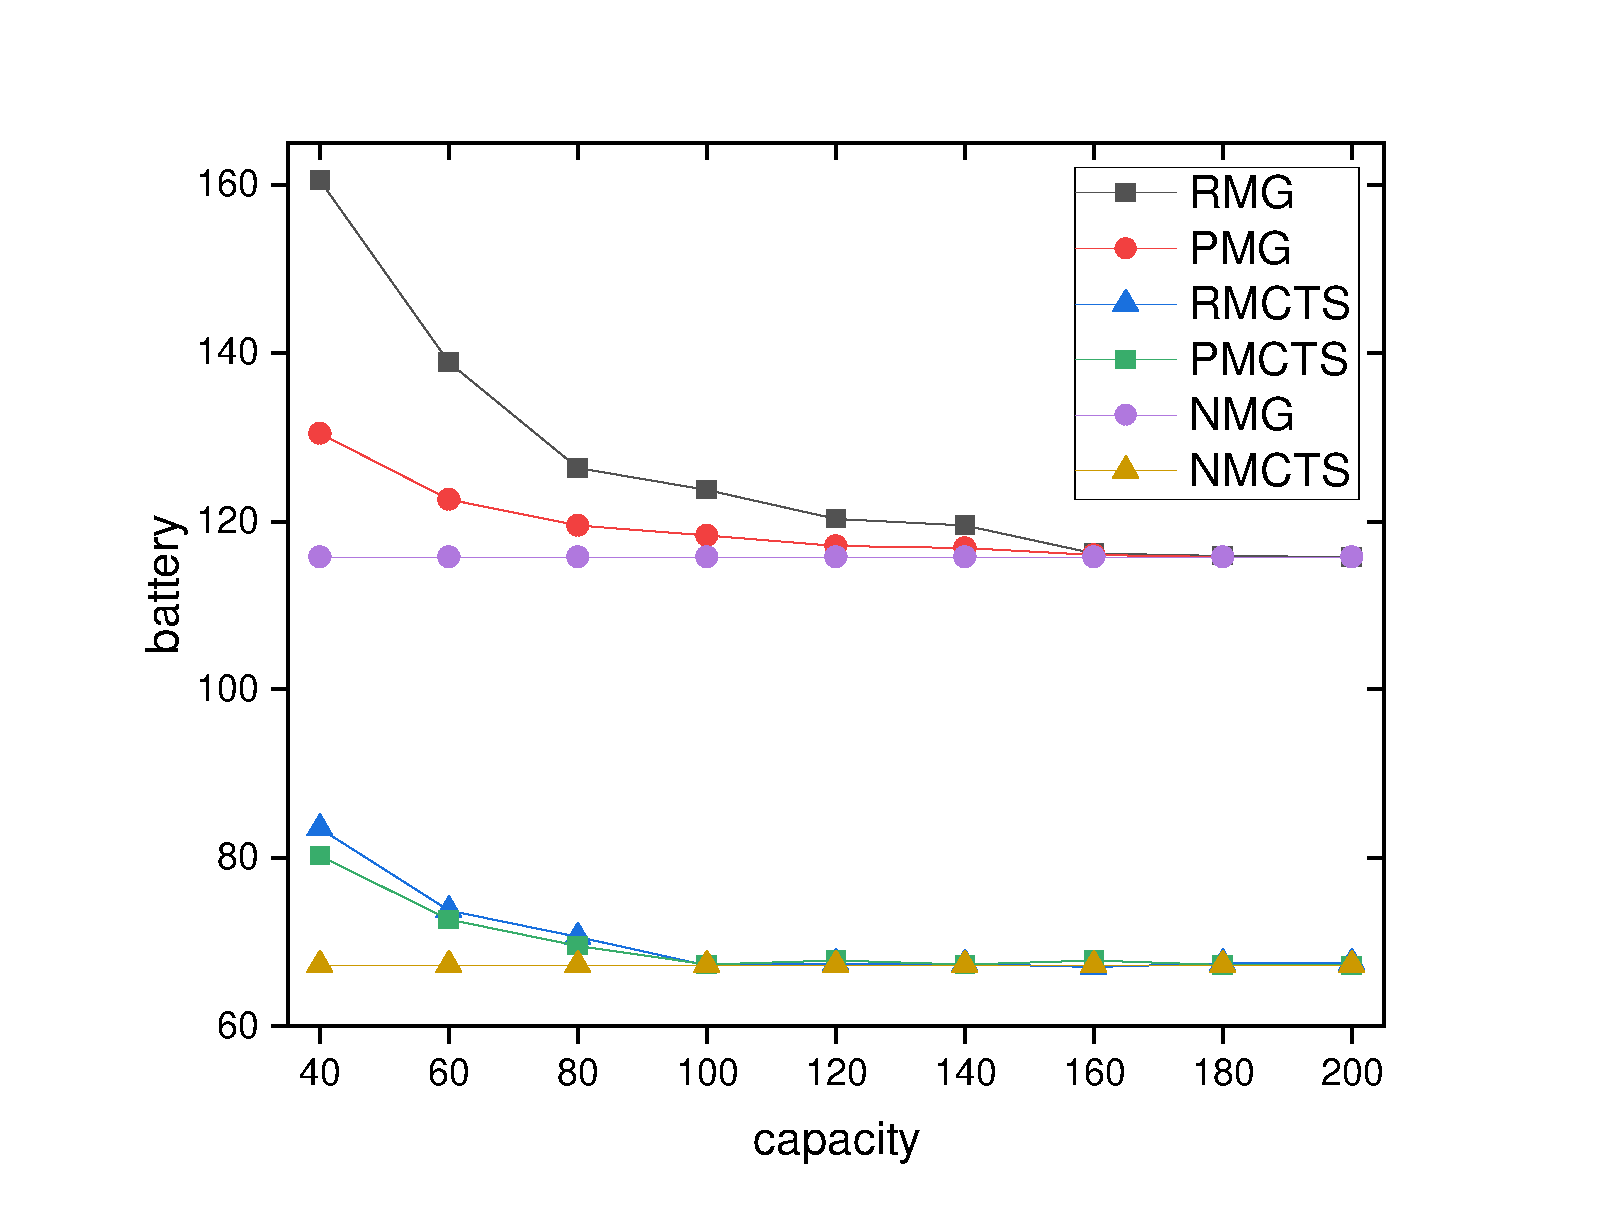
\includegraphics[scale=0.4]{./figs/cX_cY_fixG10}
\captionsetup{justification=centering}
\caption{Battery consumptions with fixed 10 goals}
\label{fig:static4}
\end{figure}

正如图中所示,当电池容量相对较低时,增加电池容量能够显著地提升所有方法的性能。
%
而当电池容量足够大时,持续地增加电池容量并不会对智能体的性能造成明显的影响。被动维持型目标和主动维持型目标在大容量电池下有非常相近的性能表现。
%
这是因为增加的电池容量会逐渐超出智能体用以实现目标的电量所需,甚至在超过一定阈值之后,提升电池容量不会对智能体性能有任何影响。然而,基于MCTS的方法在所有测试情况下都优于其他非MCTS方法。

\subsubsection{动态环境实验}
为了探究不同方法在动态环境下的性能表现,以下实验假定并非所有目标都在初始时给定。相反,一些目标会在运行时分配给智能体。
%
本实验使用变量$n$来代表两个目标的分配时间间隔。即每隔$n$周期给智能体分配一个新的目标(假定执行一个动作对应一个周期)。

\paragraph{Experiment 4}
和实验一类似,在该实验中智能体的电池容量被设定为40,实现目标的数量从1变化至15。另外,$n$的值被设定为5,也就是说每隔5个周期给智能体分配一个新的目标。
\begin{figure}[h!]
\centering
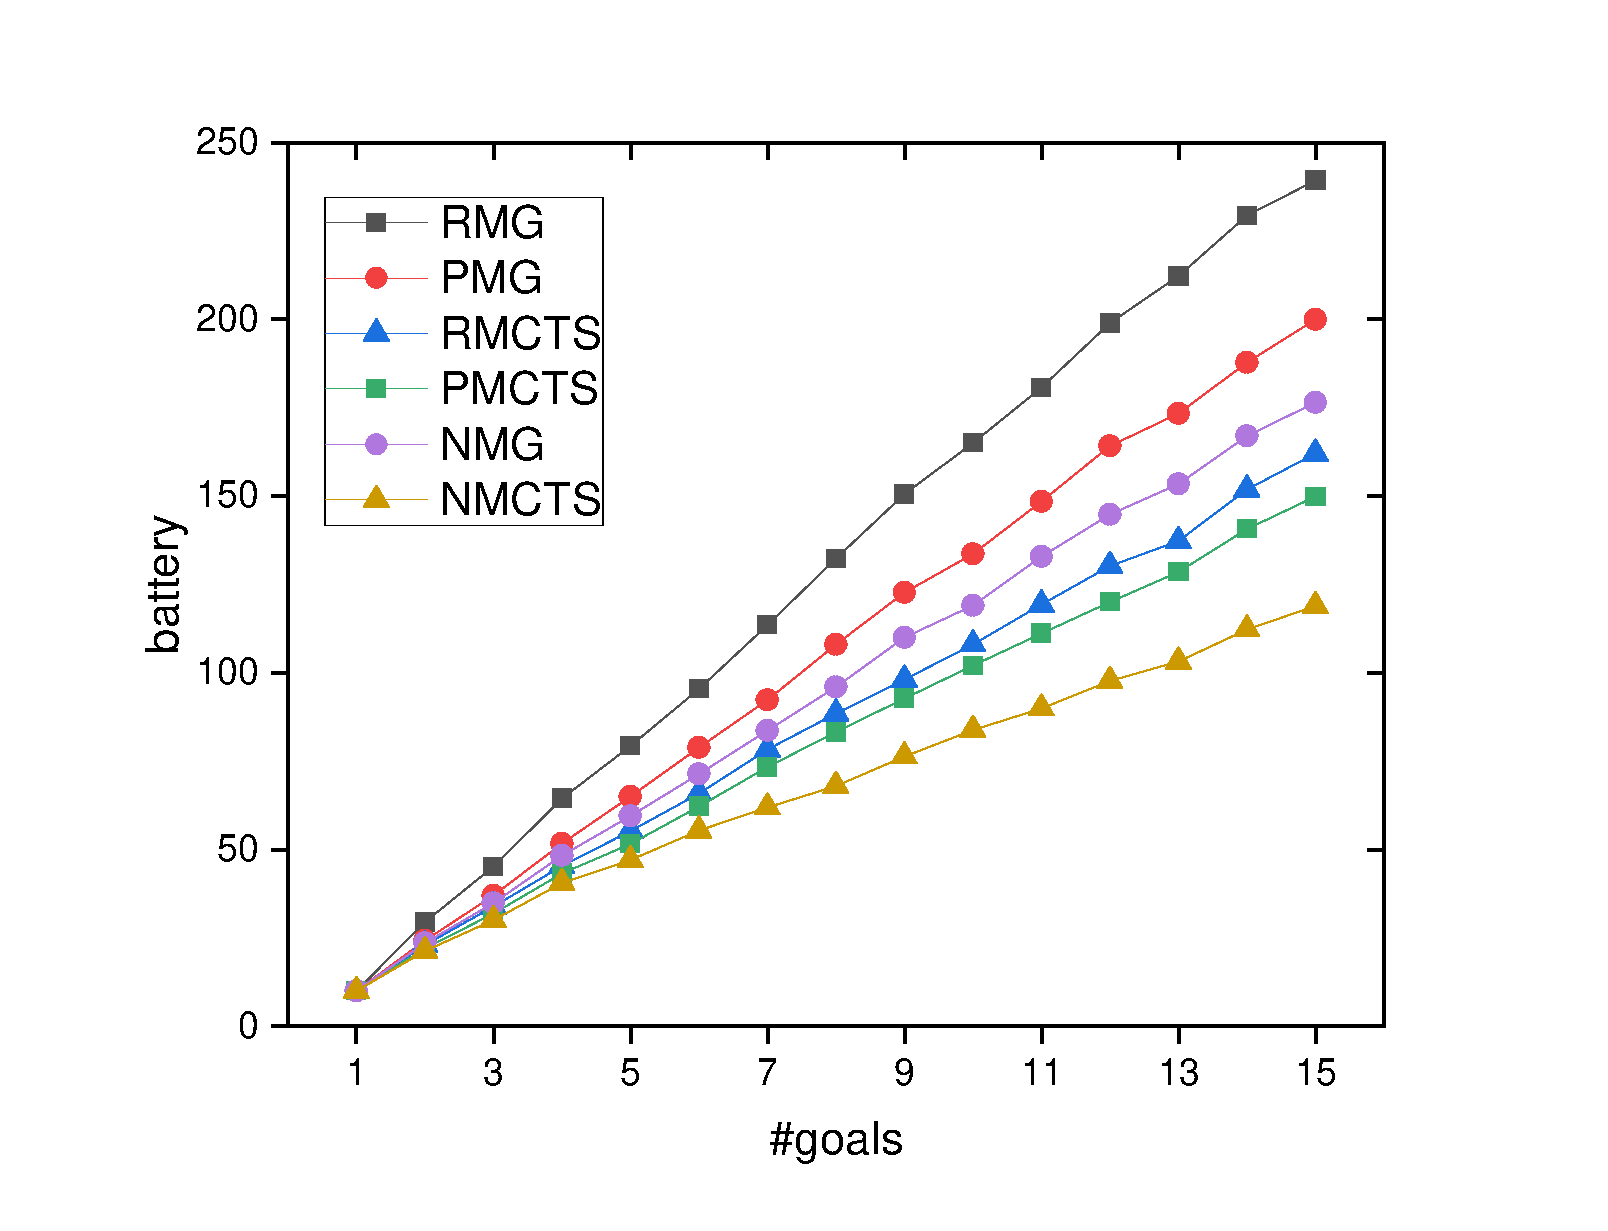
\includegraphics[scale=0.4]{./figs/gX_cY_fixCap40_d}
\captionsetup{justification=centering}
\caption{Battery consumptions with capacity of 40 in dynamic environment}
\label{fig:dynamic1}
\end{figure}

图\ref{fig:dynamic1} 展示了每个方法的平均电量消耗。
%
如图中所见,实验结果与实验一非常类似。
%
NMG,RMG和PMG的性能保持不变,而基于MCTS的方法则有较为明显的性能下降。这是因为即使目标是在不同时间分配的,非MCTS方法的执行规则并没有受到影响,仍然是依次实现给定的目标。但是基于MCTS的方法却无法预测接下来何时会有新目标的分配以及新目标指定的具体位置在何处。基于MCTS的方法只能够基于对环境当前的认知以得出”最优“的决策。
%
然而,相较于其他方法,基于MCTS的方法仍然有显著的性能优势。

\paragraph{Experiment 5}
和实验二类似,在该实验中智能体的电池容量被设定为60,实现目标的数量从1变化至15。另外,$n$的值被设定为5。
具体实验结果如图\ref{fig:dynamic2}所示.
\begin{figure}[h!]
\centering
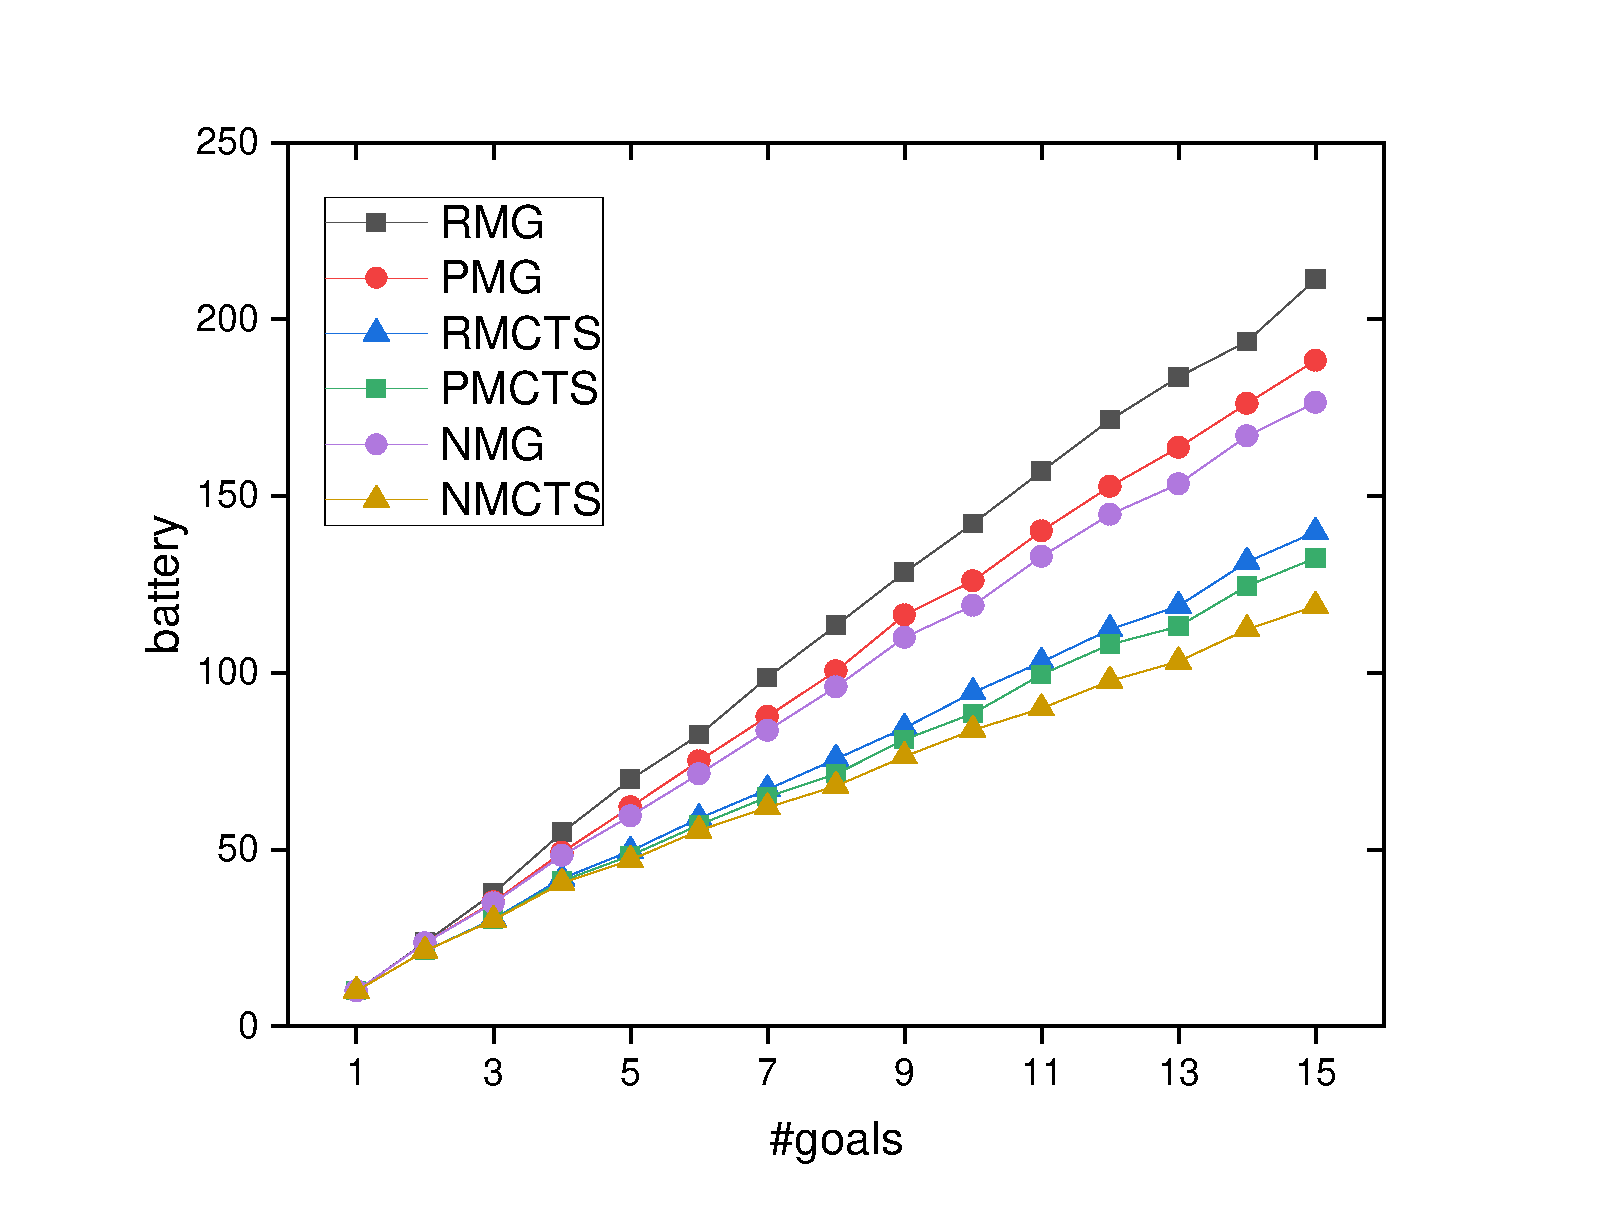
\includegraphics[scale=0.4]{./figs/gX_cY_fixCap60_d}
\captionsetup{justification=centering}
\caption{Battery consumptions with capacity of 60}
\label{fig:dynamic2}
\end{figure}

正如所预料的,该实验结果与实验二类似。相较于其他方法,基于MCTS的方法有着显著的性能优势。PMG的表现要优于RMG,但是仍然比基于MCTS的方法要消耗更多的电量,尤其是当实现目标的数量较大时。
%
另外,相较于实验二,基于MCTS的方法间的性能差异有所减小。这是由于在动态环境下智能体需要更多地考虑维持型目标的维护以及修复,导致他们的行为都更趋近于RMCTS,而对于不同意图间协同效应的利用则有所降低。

\paragraph{Experiment 6}
在实验六中,智能体实现目标的数量被固定位10,电池容量被固定为40,分配目标的时间间隔$n$从1改变至15。
\begin{figure}[h!]
\centering
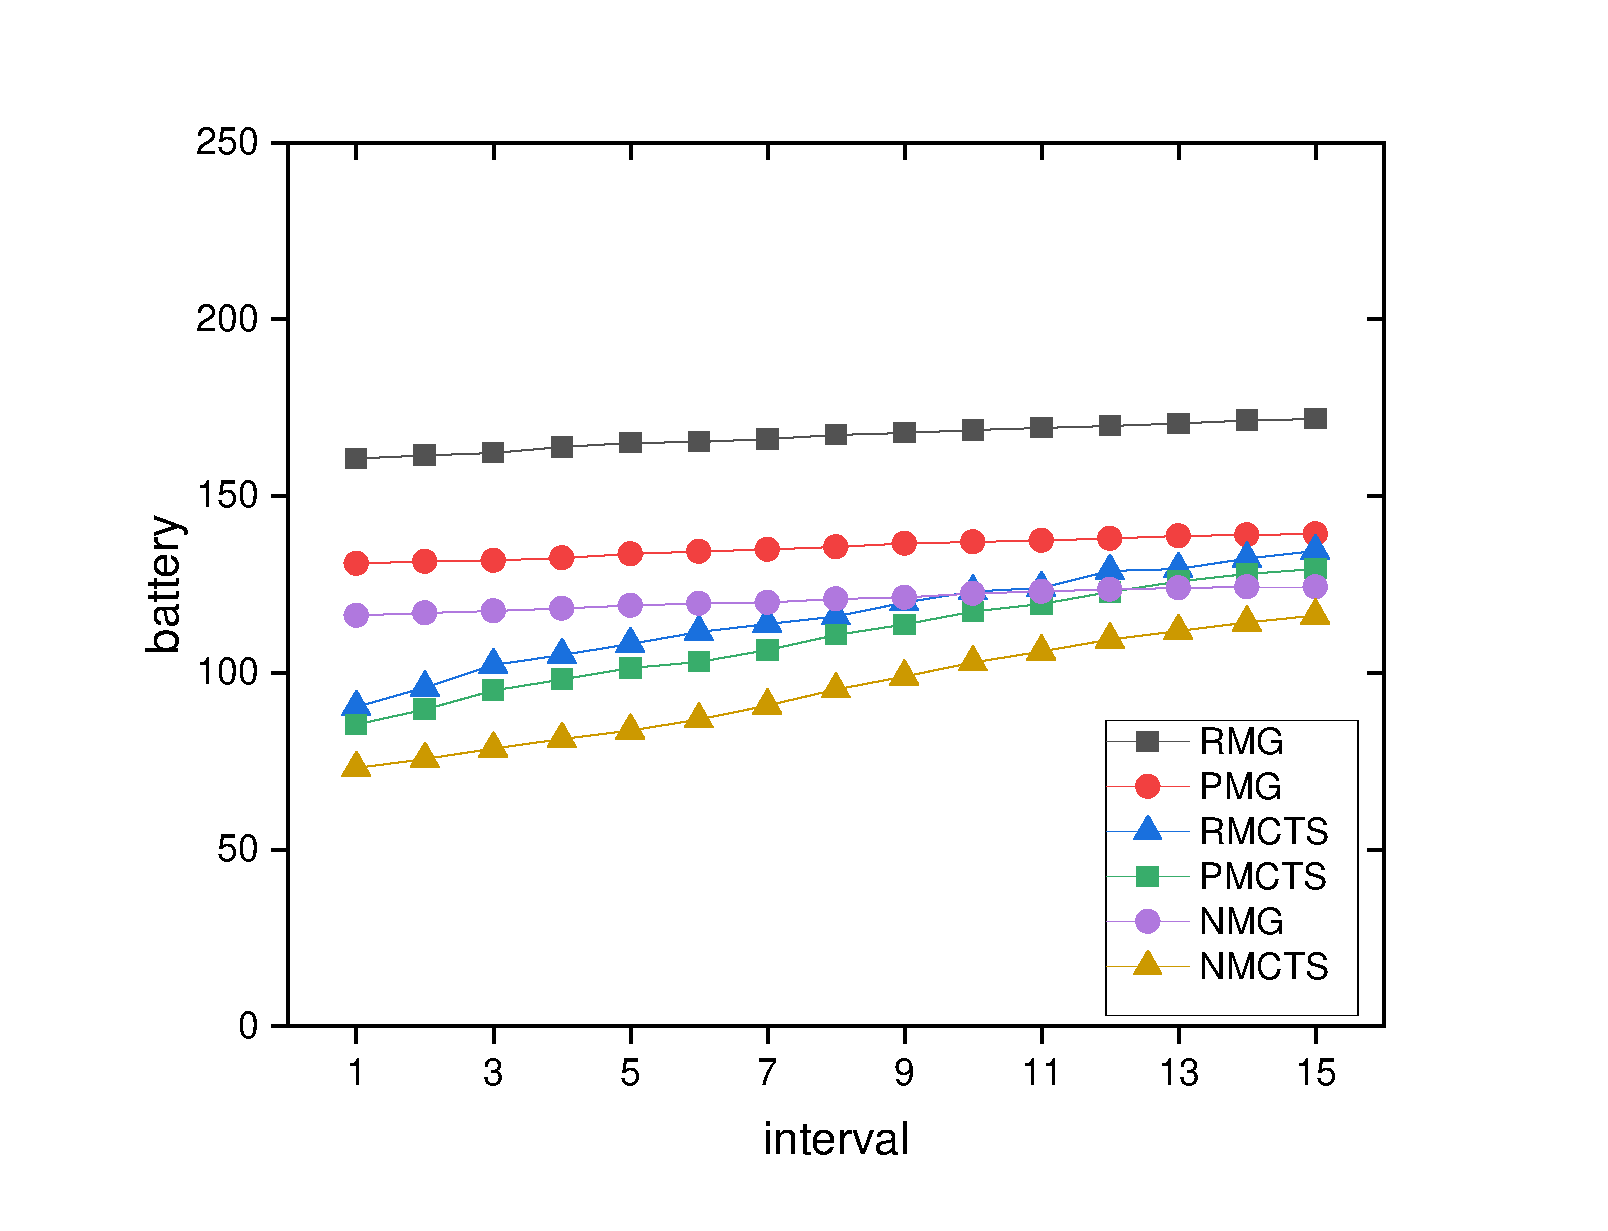
\includegraphics[scale=0.4]{./figs/iX_cY_fixCap40G10}
\captionsetup{justification=centering}
\caption{Battery consumption of different types of agents with capacity of 40 and 10 goals}
\label{fig:dynamic3}
\end{figure}

图\ref{fig:dynamic3}展示了每个方法的平均电量消耗。从图中可得知,基于MCTS方法的性能表现依然要优于其他非MCTS方法。然而,当时间间隔$n$增大时,MCTS是方法的优势越来越低。这是因为当$n$较大时,同时执行的目标数量少,MCTS方法更难以利用不同意图之间的协同效应,致使性能下降;而在$n$较小时,并发执行的意图较多,智能体可以高效利用他们之间的协同效应。当时间间隔被设定为15时,智能体在大多是情况下运行时只有一个目标,因此,MCTS的性能与其他方法非常接近。
\subsection{总结}
本章提出了一种基于MCTS的意图调度算法SAM。SAM可以同时对实现型和维持型目标进行意图调度。另外,基于火星探测器的模拟场景,本章在静态环境以及动态环境下对SAM的性能进行了分析。实验结果表明SAM与其他方法(RMG和PMG)相比有着显著的性能优势。即使在没有可靠的预测机制的情况下,SAM对被动维持型目标的调度性能表现依旧要优于其他非MCTS方法。SAM算法的主要优势有2个:1.避免维持型目标和实现型目标间的相互冲突;2.对多个意图进行交错执行以避免相互冲突并利用其协同效应。

本文的下一章将考虑如何基于MCTS,在norm约束场景下对智能体意图进行合理调度。
